\documentclass{article}
\usepackage[utf8]{inputenc}

\title{Cosmological Evidences of Dark Matter through the CMB}
\author{Lorenzo Speri}
\date{}

\usepackage{natbib}
\usepackage{graphicx}

\begin{document}

\maketitle


\section{Introduction}
-\citep{WayneHu} brief thermal history of the universe and how to get to the cmb and what is it?\\
-practical Motivation for studyinbg the cmb: nice spectrum black body spectrum: physics well know, very intense radiation\\
which info can we get from the cmb: Big bang, maater and energy content of the universe---dark matter is a big part of the matter content it influenced the spectrum  of the CMB ---- so it played a role.\\
-structure of the paper \\



%The recent measurements of the Cosmic Microwave Background (CMB) radiation allowed us to infer the presence of Dark Matter in the Universe. In this summary we will explain qualitatively how the presence of Dark Matter influences the CMB anisotropies.

\section{From the Discovery of the CMB to the Planck mission}
\citep{bucherPhysicsCosmicMicrowave2015}
-discovery of the cmb\\
-filterng of the images\\
-different missions\\

\section{Content of the Universe}
\begin{itemize}
\item Assumptions: working with the $\Lambda$CDM model
\item General relativty
\item Friedmann equations
\end{itemize}

\section{CMB theo analysis}
\begin{itemize}
\item hydrodynamics \citep{huLectureNotesCMB2008}
page 14 eq 49 to page 17 eq 71\\
skip doppler effect
\item gravito acoustic oscillations page 19 up to eq 82 , justify briefly constant potential in page 20
% if stress perturbations are negligible compared with density perturbations ( δp ≪ δρ ) then the potential will remain constant in periods where the background equation of state p/ρ is constant
\item page 20 and 21 up to eq92 important comment 
%The consequence is that overdense regions where Ψ is negative (potential wells) are cold spots in the effective temperature.
\item baryonic effect
\end{itemize}
hydrodinamics







\begin{figure}[h!]
\centering
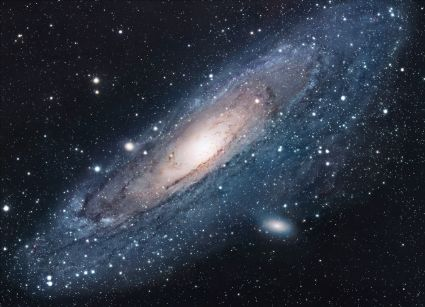
\includegraphics[scale=1.7]{universe}
\caption{The Universe}
\label{fig:universe}
\end{figure}

\section{Conclusion}
nn
\citep{padmanabhanDetectingDarkMatter2005}



\bibliographystyle{plain}
\bibliography{dark}
\end{document}
